\documentclass[10pt, a4paper]{article}

% --- 基础宏包 ---
\usepackage[margin=2.5cm]{geometry} % 设置页面边距
\usepackage{amsmath, amssymb}       % 数学公式支持
\usepackage{fancyhdr}               % 页眉页脚支持
\usepackage{ctex}
\usepackage{enumitem}
\usepackage{array}
\usepackage{tikz}
\usepackage{booktabs}
\usepackage{float}
\usetikzlibrary{shapes.geometric}
\usetikzlibrary{shapes.gates.logic.US,arrows.meta,positioning}

\setlist[enumerate]{label=(\arabic*), nosep}
\setlist[itemize]{nosep}

% --- 页眉页脚设置 ---
\pagestyle{fancy}
\fancyhf{}							% 清空默认的页眉页脚
\lhead{数字逻辑电路}                 % 左侧页眉
\rhead{19Q24119 汤今越}              % 右侧页眉
\cfoot{第 \thepage\ 页}              % 底部居中页码
\setlength{\headheight}{15pt}       % 调整页眉高度以避免警告

% --- 自定义题目与解答命令 ---
% #1: 题号, #2: 题目内容 (\kaishu 切换为楷体)
\newcommand{\question}[2]{
    \vspace{2ex}\noindent\textbf{#1}\ {\kaishu #2} \par\vspace{1ex}
}
% #1: 解答内容 (\songti 切换为宋体)
\newcommand{\solution}[1]{
    \noindent\textbf{解：}{\songti #1} \par\vspace{3ex}
}

\begin{document}

% ================= 表头信息 =================
\thispagestyle{plain}
\begin{center}
	\hrule
	\vspace{.4cm}
	{\textbf { \large 数字逻辑电路\ 作业}}
\end{center}
{ \textbf{姓名：}}汤今越 \hspace{\fill} \textbf{日期:} 2026-03-27 \\
{ \textbf{学号：}}19Q24119 \hspace{\fill} \textbf{作业编号:} 03 \\
	\hrule
\vspace{3ex}
% ============================================

% ================= 作业内容 =================

\question{3.11 \& 3.12}{
写出下列各式的最小项和最大项表达式。
\begin{enumerate}
	\item $ F = A\overline{C} + \overline{A}C + BC $
	\item $ F = A\overline{B} + \overline{A}B + BCD $
	\item $ F = ABC + ABCD + A\overline{D} $
	\item $ F = ABC + ACD + B\overline{D} + \overline{A}C $
	\item $ F = (C + \overline{A}B) [ (\overline{A} + B) \cdot C + A] $
	\item $ F = \overline{\overline{\overline{AC + B} + CD} + \overline{A}\,\overline{D}} + \overline{\overline{C} + \overline{B}} $
\end{enumerate}
}

\solution{
最小项：
\begin{enumerate}
	\item $ F = \sum m(1,3,4,6,7) $
	\item $ F = \sum m(4,5,6,7,8,9,10,11,15) $
	\item $ F = \sum m(8,10,12,14,15) $
	\item $ F = \sum m(2,3,4,6,7,11,12,14,15) $
	\item $ F = \sum m(1,3,5,7) $
	\item $ F = \sum m(1,3,6,7,8,9,11,14,15) $
\end{enumerate}
最大项：
\begin{enumerate}
	\item $ F = \prod M(0,2,5) $
	\item $ F = \prod M(0,1,2,3,12,13,14) $
	\item $ F = \prod M(0,1,2,3,4,5,6,7,9,11,13) $
	\item $ F = \prod M(0,1,5,8,9,10,13) $
	\item $ F = \prod M(0,2,4,6) $
	\item $ F = \prod M(0,2,4,5,10,12,13) $ 
\end{enumerate}
}

\question{3.14 \& 3.15}{
作下列函数的卡诺图、反函数的卡诺图，写出反函数。
\begin{enumerate}
    \item[(1)] $Y = \overline{B + \overline{A} \cdot \overline{C}}$
    \item[(3)] $Y = (\overline{B} + A)(B + C + D)(\overline{A} + \overline{C})$
    \item[(5)] $Y = \sum m(0, 1, 2, 3, 4, 9, 14, 15)$
    \item[(7)] $Y = f(A, B, C) = \prod M(0, 2, 4, 6)$
\end{enumerate}
}

\solution{
\begin{enumerate}
\item[(1)] $Y = \overline{B + \overline{A} \cdot \overline{C}}$

$Y$ 的卡诺图：
\[
\begin{array}{c|cccc}
A\backslash BC  & 00 & 01 & 11 & 10 \\ \hline
0 & 0 & 1 & 0 & 0 \\
1 & 1 & 1 & 0 & 0 
\end{array}
\]

其反函数 $\overline{Y}$ 的卡诺图（原卡诺图中1变0、0变1）：
\[
\begin{array}{c|cccc}
A\backslash BC  & 00 & 01 & 11 & 10 \\ \hline
0 & 1 & 0 & 1 & 1 \\
1 & 0 & 0 & 1 & 1 
\end{array}
\]
$\overline{Y} = \sum m(0,2,3,6,7)$

\item[(3)] $Y = (\overline{B} + A)(B + C + D)(\overline{A} + \overline{C})$

$Y$ 的卡诺图：
\[
\begin{array}{c|cccc}
AB\backslash CD & 00 & 01 & 11 & 10 \\ \hline
00 & 0 & 1 & 1 & 1 \\
01 & 0 & 0 & 0 & 0 \\
11 & 1 & 1 & 0 & 0 \\
10 & 0 & 1 & 0 & 0 
\end{array}
\]

其反函数 $\overline{Y}$ 的卡诺图：
\[
\begin{array}{c|cccc}
AB\backslash CD & 00 & 01 & 11 & 10 \\ \hline
00 & 1 & 0 & 0 & 0 \\
01 & 1 & 1 & 1 & 1 \\
11 & 0 & 0 & 1 & 1 \\
10 & 1 & 0 & 1 & 1 
\end{array}
\]
$\overline{Y} = \sum m(0,4,5,6,7,8,10,11,14,15)$

\item[(5)] $Y = \sum m(0,1,2,3,4,9,14,15)$

$Y$ 的卡诺图：
\[
\begin{array}{c|cccc}
AB\backslash CD & 00 & 01 & 11 & 10 \\ \hline
00 & 1 & 1 & 1 & 1 \\
01 & 1 & 0 & 0 & 0 \\
11 & 0 & 0 & 1 & 1 \\
10 & 0 & 1 & 0 & 0 
\end{array}
\]

其反函数 $\overline{Y}$ 的卡诺图：
\[
\begin{array}{c|cccc}
AB\backslash CD & 00 & 01 & 11 & 10 \\ \hline
00 & 0 & 0 & 0 & 0 \\
01 & 0 & 1 & 1 & 1 \\
11 & 1 & 1 & 0 & 0 \\
10 & 1 & 0 & 1 & 1 
\end{array}
\]
$\overline{Y} = \sum m(5,6,7,8,10,11,12,13)$

\item[(7)] $Y = f(A,B,C) = \prod M(0,2,4,6)$

$Y$ 的卡诺图：
\[
\begin{array}{c|cccc}
A\backslash BC & 00 & 01 & 11 & 10 \\ \hline
0 & 0 & 1 & 1 & 0 \\
1 & 0 & 1 & 1 & 0 
\end{array}
\]

其反函数 $\overline{Y}$ 的卡诺图：
\[
\begin{array}{c|cccc}
A\backslash BC & 00 & 01 & 11 & 10 \\ \hline
0 & 1 & 0 & 0 & 1 \\
1 & 1 & 0 & 0 & 1 
\end{array}
\]
$\overline{Y} = \sum m(0,2,4,6)$
\end{enumerate}
}

\question{3.21 \& 3.22 \& 3.23}{
用卡诺图简化下列各函数，写出函数的最简{\heiti{与-或、或-与、与-或非}}表达式。
\begin{enumerate}
    \item[(2)] $F = \overline{A}C + \overline{C}D + BC + AD$
    \item[(4)] $F = (\overline{A}+B)(\overline{A}+B+C)(A+C)(A+C+D)$
    \item[(6)] $F = f(A, B, C, D) = \sum m(0, 2, 5, 7, 9, 10) + \sum d(1, 4, 8, 12, 15)$
    \item[(8)] $F = f(A, B, C, D) = \prod M(0, 2, 5, 7, 9, 10) \cdot \prod d(1, 4, 8, 12, 15)$
\end{enumerate}
}

\solution{
\textbf{卡诺图}

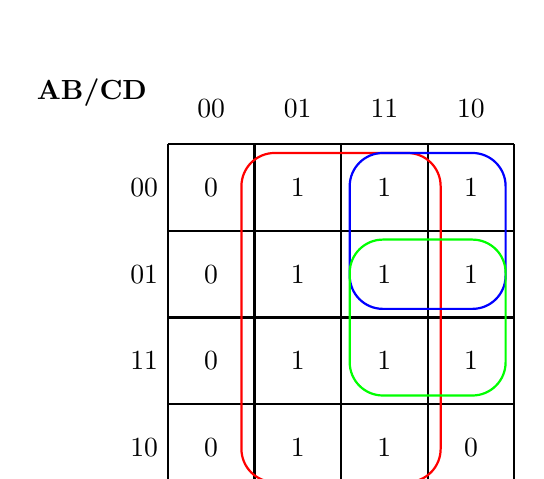
\begin{tikzpicture}[scale=1.1]
  % 网格
  \draw[step=1cm, thick] (0,0) grid (4,4);
  
  % 列标签 CD（上方）
  \node[above] at (0.5,4.2) {00};
  \node[above] at (1.5,4.2) {01};
  \node[above] at (2.5,4.2) {11};
  \node[above] at (3.5,4.2) {10};
  \node[above left=0.2cm] at (0,4.2) {\textbf{AB/CD}};
  
  % 行标签 AB（左侧）
  \node[left] at (0,3.5) {00};
  \node[left] at (0,2.5) {01};
  \node[left] at (0,1.5) {11};
  \node[left] at (0,0.5) {10};
  %\node[rotate=90, left=0.2cm] at (0,4) {\textbf{AB}};
  
  % 单元格数值（从上到下：AB=00→01→11→10）
  \node at (0.5,3.5) {0};
  \node at (1.5,3.5) {1};
  \node at (2.5,3.5) {1};
  \node at (3.5,3.5) {1};
  
  \node at (0.5,2.5) {0};
  \node at (1.5,2.5) {1};
  \node at (2.5,2.5) {1};
  \node at (3.5,2.5) {1};
  
  \node at (0.5,1.5) {0};
  \node at (1.5,1.5) {1};
  \node at (2.5,1.5) {1};
  \node at (3.5,1.5) {1};
  
  \node at (0.5,0.5) {0};
  \node at (1.5,0.5) {1};
  \node at (2.5,0.5) {1};
  \node at (3.5,0.5) {0};
  
  % 分组圈出（多颜色）
  % 红色：D（CD=01和11两整列，4×2=8格）
  \draw[thick, red, rounded corners=12pt] (0.85,0.1) rectangle (3.15,3.9);
  
  % 蓝色：$\overline{A}C$（AB=00、01两行 + CD=11、10两列，2×2=4格）
  \draw[thick, blue, rounded corners=12pt] (2.1,2.1) rectangle (3.9,3.9);
  
  % 绿色：$BC$（AB=01、11两行 + CD=11、10两列，2×2=4格）
  \draw[thick, green, rounded corners=12pt] (2.1,1.1) rectangle (3.9,2.9);
\end{tikzpicture}

\textbf{最简与-或表达式：} $F = \overline{A}C + BC + D$

\textbf{最简或-与表达式：} $F = (C + D)(\overline{A} + B + D)$

\textbf{最简与-或非表达式：} $F = \overline{\overline{\overline{A}C} \cdot \overline{BC} \cdot \overline{D}}$

\subsection*{(4) $F = (\overline{A}+B)(\overline{A}+B+C)(A+C)(A+C+D)$}

\textbf{卡诺图}

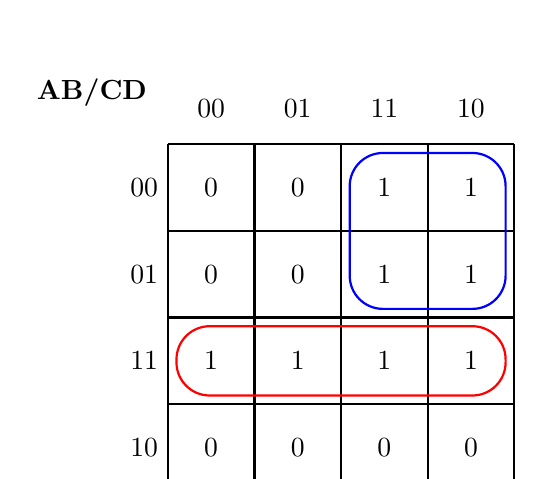
\begin{tikzpicture}[scale=1.1]
  % 网格
  \draw[step=1cm, thick] (0,0) grid (4,4);
  
  % 列标签 CD
  \node[above] at (0.5,4.2) {00};
  \node[above] at (1.5,4.2) {01};
  \node[above] at (2.5,4.2) {11};
  \node[above] at (3.5,4.2) {10};
  \node[above left=0.2cm] at (0,4.2) {\textbf{AB/CD}};
  
  % 行标签 AB
  \node[left] at (0,3.5) {00};
  \node[left] at (0,2.5) {01};
  \node[left] at (0,1.5) {11};
  \node[left] at (0,0.5) {10};
  %\node[rotate=90, left=0.2cm] at (0,4) {\textbf{AB}};
  
  % 单元格数值
  \node at (0.5,3.5) {0};
  \node at (1.5,3.5) {0};
  \node at (2.5,3.5) {1};
  \node at (3.5,3.5) {1};
  
  \node at (0.5,2.5) {0};
  \node at (1.5,2.5) {0};
  \node at (2.5,2.5) {1};
  \node at (3.5,2.5) {1};
  
  \node at (0.5,1.5) {1};
  \node at (1.5,1.5) {1};
  \node at (2.5,1.5) {1};
  \node at (3.5,1.5) {1};
  
  \node at (0.5,0.5) {0};
  \node at (1.5,0.5) {0};
  \node at (2.5,0.5) {0};
  \node at (3.5,0.5) {0};
  
  % 分组圈出
  % 红色：$AB$（AB=11整行，1×4=4格）
  \draw[thick, red, rounded corners=12pt] (0.1,1.1) rectangle (3.9,1.9);
  
  % 蓝色：$\overline{A}C$（AB=00、01两行 + CD=11、10两列，2×2=4格）
  \draw[thick, blue, rounded corners=12pt] (2.1,2.1) rectangle (3.9,3.9);
\end{tikzpicture}

\textbf{最简与-或表达式：} $F = AB + \overline{A}C$

\textbf{最简或-与表达式：} $F = (A + C)(B + \overline{A})$

\textbf{最简与-或非表达式：} $F = \overline{\overline{AB} \cdot \overline{\overline{A}C}}$

\subsection*{(6) $F = f(A, B, C, D) = \sum m(0, 2, 5, 7, 9, 10) + \sum d(1, 4, 8, 12, 15)$}

\textbf{卡诺图}

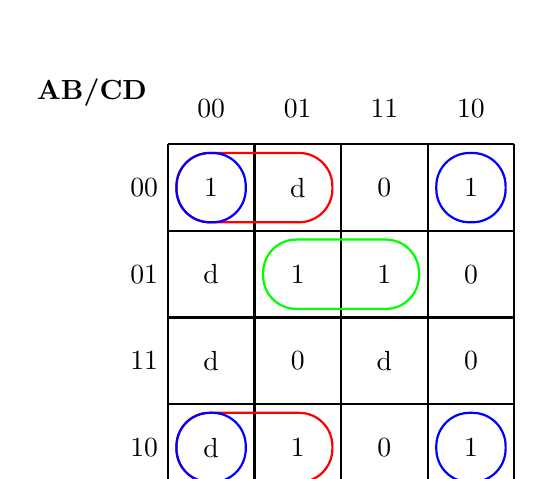
\begin{tikzpicture}[scale=1.1]
  % 网格
  \draw[step=1cm, thick] (0,0) grid (4,4);
  
  % 列标签 CD
  \node[above] at (0.5,4.2) {00};
  \node[above] at (1.5,4.2) {01};
  \node[above] at (2.5,4.2) {11};
  \node[above] at (3.5,4.2) {10};
  \node[above left=0.2cm] at (0,4.2) {\textbf{AB/CD}};
  
  % 行标签 AB
  \node[left] at (0,3.5) {00};
  \node[left] at (0,2.5) {01};
  \node[left] at (0,1.5) {11};
  \node[left] at (0,0.5) {10};
  %\node[rotate=90, left=0.2cm] at (0,4) {\textbf{AB}};
  
  % 单元格数值
  \node at (0.5,3.5) {1};
  \node at (1.5,3.5) {d};
  \node at (2.5,3.5) {0};
  \node at (3.5,3.5) {1};
  
  \node at (0.5,2.5) {d};
  \node at (1.5,2.5) {1};
  \node at (2.5,2.5) {1};
  \node at (3.5,2.5) {0};
  
  \node at (0.5,1.5) {d};
  \node at (1.5,1.5) {0};
  \node at (2.5,1.5) {d};
  \node at (3.5,1.5) {0};
  
  \node at (0.5,0.5) {d};
  \node at (1.5,0.5) {1};
  \node at (2.5,0.5) {0};
  \node at (3.5,0.5) {1};
  
  % 分组圈出（多颜色）
  % 红色：$\overline{B}\overline{C}$（B=0的两行 + C=0的两列，含d，2×2=4格，上下包络）
  \draw[thick, red, rounded corners=12pt] (0.1,3.1) rectangle (1.9,3.9); % 上部
  \draw[thick, red, rounded corners=12pt] (0.1,0.1) rectangle (1.9,0.9);   % 下部（环绕）
  
  % 蓝色：$\overline{B}\overline{D}$（B=0的两行 + D=0的两列，含d，2×2环绕四角）
  \draw[thick, blue, rounded corners=12pt] (0.1,3.1) rectangle (0.9,3.9); % 左上
  \draw[thick, blue, rounded corners=12pt] (3.1,3.1) rectangle (3.9,3.9); % 右上
  \draw[thick, blue, rounded corners=12pt] (0.1,0.1) rectangle (0.9,0.9); % 左下
  \draw[thick, blue, rounded corners=12pt] (3.1,0.1) rectangle (3.9,0.9); % 右下
  
  % 绿色：$\overline{A}BD$（AB=01一行 + D=1的两列，2格）
  \draw[thick, green, rounded corners=12pt] (1.1,2.1) rectangle (2.9,2.9);
\end{tikzpicture}

\textbf{最简与-或表达式：} $F = \overline{B}\overline{C} + \overline{B}\overline{D} + \overline{A}BD$

\textbf{最简或-与表达式：} $F = (D + \overline{B})(\overline{A} + \overline{B})(B + \overline{C} + \overline{D})$

\textbf{最简与-或非表达式：} $F = \overline{\overline{\overline{B}\overline{C}} \cdot \overline{\overline{B}\overline{D}} \cdot \overline{\overline{A}BD}}$

\subsection*{(8) $F = f(A, B, C, D) = \prod M(0, 2, 5, 7, 9, 10) \cdot \prod d(1, 4, 8, 12, 15)$}

\textbf{卡诺图}

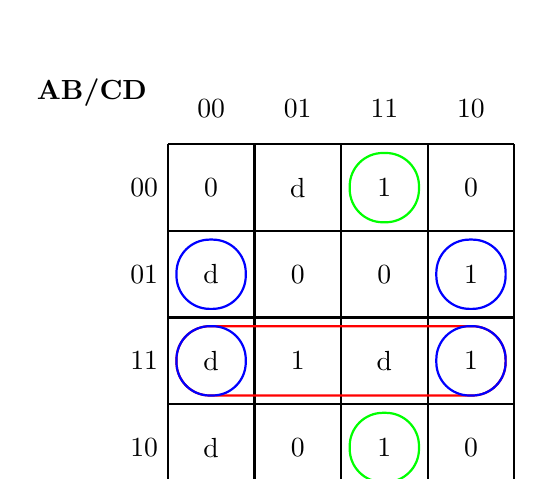
\begin{tikzpicture}[scale=1.1]
  % 网格
  \draw[step=1cm, thick] (0,0) grid (4,4);
  
  % 列标签 CD
  \node[above] at (0.5,4.2) {00};
  \node[above] at (1.5,4.2) {01};
  \node[above] at (2.5,4.2) {11};
  \node[above] at (3.5,4.2) {10};
  \node[above left=0.2cm] at (0,4.2) {\textbf{AB/CD}};
  
  % 行标签 AB
  \node[left] at (0,3.5) {00};
  \node[left] at (0,2.5) {01};
  \node[left] at (0,1.5) {11};
  \node[left] at (0,0.5) {10};
  %\node[rotate=90, left=0.2cm] at (0,4) {\textbf{AB}};
  
  % 单元格数值
  \node at (0.5,3.5) {0};
  \node at (1.5,3.5) {d};
  \node at (2.5,3.5) {1};
  \node at (3.5,3.5) {0};
  
  \node at (0.5,2.5) {d};
  \node at (1.5,2.5) {0};
  \node at (2.5,2.5) {0};
  \node at (3.5,2.5) {1};
  
  \node at (0.5,1.5) {d};
  \node at (1.5,1.5) {1};
  \node at (2.5,1.5) {d};
  \node at (3.5,1.5) {1};
  
  \node at (0.5,0.5) {d};
  \node at (1.5,0.5) {0};
  \node at (2.5,0.5) {1};
  \node at (3.5,0.5) {0};
  
  % 分组圈出（多颜色）
  % 红色：$AB$（AB=11整行，含d，1×4=4格）
  \draw[thick, red, rounded corners=12pt] (0.1,1.1) rectangle (3.9,1.9);
  
  % 蓝色：$B\overline{D}$（B=1的两行 + D=0的两列，含d，2×2环绕）
  \draw[thick, blue, rounded corners=12pt] (0.1,1.1) rectangle (0.9,1.9); % 左
  \draw[thick, blue, rounded corners=12pt] (0.1,2.1) rectangle (0.9,2.9);
  \draw[thick, blue, rounded corners=12pt] (3.1,1.1) rectangle (3.9,1.9); % 右
  \draw[thick, blue, rounded corners=12pt] (3.1,2.1) rectangle (3.9,2.9);
  
  % 绿色：$\overline{B}CD$（B=0的两行 + CD=11一列，含环绕，2格）
  \draw[thick, green, rounded corners=12pt] (2.1,3.1) rectangle (2.9,3.9); % 上
  \draw[thick, green, rounded corners=12pt] (2.1,0.1) rectangle (2.9,0.9);   % 下（环绕）
\end{tikzpicture}

\textbf{最简与-或表达式：} $F = AB + B\overline{D} + \overline{B}CD$

\textbf{最简或-与表达式：} $F = (B + C)(B + D)(A + \overline{B} + \overline{D})$

\textbf{最简与-或非表达式：} $F = \overline{\overline{AB} \cdot \overline{B\overline{D}} \cdot \overline{\overline{B}CD}}$
}

\question{5.3}{
写出所示的两个电路的逻辑表达式和真值表。
}

\solution{
\begin{itemize}
	\item a 电路逻辑表达式
	
	$ Y_1 = \overline{A\overline{B}} = \overline{A} + B $

	$ Y_3 = \overline{\overline{B} + \overline{C}} = BC $

	$ Y_2 = \overline{\overline{AC} + Y_3} = A\overline{B}\,\overline{C} + \overline{A}BC$

	\item a 电路真值表

	\begin{table}[h]
		\centering
		\begin{tabular}{ccc|ccc}
		\toprule
		A & B & C & $Y_1$ & $Y_3$ & $Y_2$ \\
		\midrule
		0 & 0 & 0 & 1 & 0 & 0 \\
		0 & 0 & 1 & 1 & 0 & 0 \\
		0 & 1 & 0 & 1 & 0 & 0 \\
		0 & 1 & 1 & 1 & 1 & 1 \\
		1 & 0 & 0 & 0 & 0 & 1 \\
		1 & 0 & 1 & 0 & 0 & 0 \\
		1 & 1 & 0 & 1 & 0 & 0 \\
		1 & 1 & 1 & 1 & 1 & 0 \\
		\bottomrule
		\end{tabular} 
	\end{table}

	\item b 电路逻辑表达式
	
	$ Y = \overline{\overline{\overline{A}\,\overline{B}C}(\overline{A} + \overline{B} + C)} = A + B + \overline{C} $

	\item b 电路真值表

	\begin{table}[h]
		\centering
		\begin{tabular}{ccc|c}
		\toprule
		A & B & C & Y \\
		\midrule
		0 & 0 & 0 & 1 \\
		0 & 0 & 1 & 0 \\
		0 & 1 & 0 & 1 \\
		0 & 1 & 1 & 1 \\
		1 & 0 & 0 & 1 \\
		1 & 0 & 1 & 1 \\
		1 & 1 & 0 & 1 \\
		1 & 1 & 1 & 1 \\
		\bottomrule
		\end{tabular}
	\end{table}
\end{itemize}
}

\question{5.4}{
用真值表、卡诺图和逻辑图（与或）表示逻辑函数 $ L=A\overline{B} + B\overline{C} + C\overline{A}
$。}

\solution{
逻辑函数：$ L = A\overline{B} + B\overline{C} + C\overline{A} $

真值表

\begin{table}[h]
	\centering
	\begin{tabular}{ccc|c}
		\toprule
		A & B & C & L \\
		\midrule
		0 & 0 & 0 & 1 \\
		0 & 0 & 1 & 0 \\
		0 & 1 & 0 & 1 \\
		0 & 1 & 1 & 1 \\
		1 & 0 & 0 & 1 \\
		1 & 0 & 1 & 1 \\
		1 & 1 & 0 & 0 \\
		1 & 1 & 1 & 1 \\
		\bottomrule
	\end{tabular}
\end{table}

卡诺图
\[
\begin{array}{c|cccc}
A\backslash BC & 00 & 01 & 11 & 10 \\ \hline
0 & 1 & 1 & 0 & 1 \\
1 & 0 & 1 & 1 & 1 
\end{array}
\]

逻辑图

\begin{figure}[h]
    \centering
    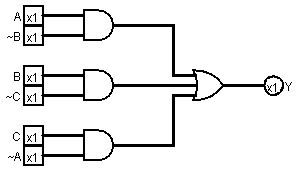
\includegraphics[width=0.3\textwidth]{5.3.png}
    \caption{5.3}
\end{figure}

}

\question{5.11}{
用与非门实现函数 $ F $，写出真值表并画出逻辑图。
$ F = \overline{\overline{A}\,\overline{B}CD + AB\overline{C}D + A\overline{B}\,\overline{C}D + A\overline{B}C\overline{D}} $
}

\solution{
$ F = \overline{A}\,\overline{C} + \overline{A}\,\overline{D} + \overline{C}\,\overline{D} + BC + ACD = \overline{\overline{\overline{A}\,\overline{C}} \cdot \overline{\overline{A}\,\overline{D}} \cdot \overline{\overline{C}\,\overline{D}} \cdot \overline{BC} \cdot \overline{ACD}} $

逻辑图

\begin{figure}[H]
    \centering
    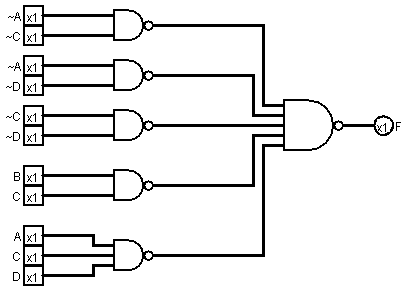
\includegraphics[width=0.3\textwidth]{5.11.png}
    \caption{5.11}
\end{figure}

真值表

\begin{table}[h]
	\centering
	\begin{tabular}{cccc|c}
		\toprule
		A & B & C & D & F \\
		\midrule
		0 & 0 & 0 & 0 & 1 \\
		0 & 0 & 0 & 1 & 1 \\
		0 & 0 & 1 & 0 & 1 \\
		0 & 0 & 1 & 1 & 0 \\
		0 & 1 & 0 & 0 & 1 \\
		0 & 1 & 0 & 1 & 1 \\
		0 & 1 & 1 & 0 & 1 \\
		0 & 1 & 1 & 1 & 1 \\
		1 & 0 & 0 & 0 & 1 \\
		1 & 0 & 0 & 1 & 0 \\
		1 & 0 & 1 & 0 & 0 \\
		1 & 0 & 1 & 1 & 1 \\
		1 & 1 & 0 & 0 & 1 \\
		1 & 1 & 0 & 1 & 0 \\
		1 & 1 & 1 & 0 & 1 \\
		1 & 1 & 1 & 1 & 1 \\
		\bottomrule
	\end{tabular}
\end{table}
}

\question{5.12}{
用或非门实现函数 $ F $，并画出逻辑图。
$ F = A\overline{B}C\overline{D} + \overline{A}BC\overline{D}+A\overline{B}\,\overline{C}D + \overline{A}B\overline{C}D $
}

\solution{
$ F = (A + B)(\overline{A} + \overline{B})(C + D)(\overline{C} + \overline{D}) = \overline{\overline{\overline{A} + \overline{B}} + \overline{A + B} + \overline{\overline{C} + \overline{D}} + \overline{C + D}} $

逻辑图

\begin{figure}[h]
    \centering
    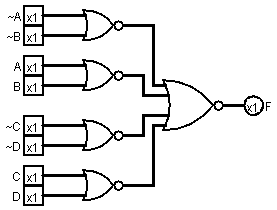
\includegraphics[width=0.3\textwidth]{5.12.png}
    \caption{5.12}
\end{figure}
}

\question{5.15}{
逻辑函数最小项表达式为$ F = \Sigma m(2,4,8,11,12,14) $，完成下列设计：
\begin{enumerate}
	\item 采用与或非门实现；
	\item 采用与非门实现。
\end{enumerate}
}

\solution{
$F = \overline{A}\,\overline{B}D + A\overline{C}\,\overline{D} + BC\overline{D} = \overline{\overline{\overline{A}\,\overline{B}D} \cdot \overline{A\overline{C}\,\overline{D}} \cdot \overline{BC\overline{D}}}$

\begin{figure}[h]
    \centering
    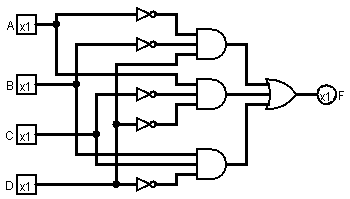
\includegraphics[width=0.3\textwidth]{5.15.1.png}
    \caption{5.15.1}
\end{figure}

\begin{figure}[h]
    \centering
    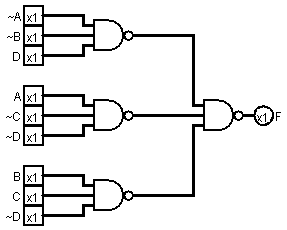
\includegraphics[width=0.3\textwidth]{5.15.2.png}
    \caption{5.15.2}
\end{figure}
}

\question{5.16}{
设计逻辑电路实现：两个2位二进制数相等时输出为\textbf{1}，不等时输出\textbf{0}。
}

\solution{
\begin{figure}[h]
    \centering
    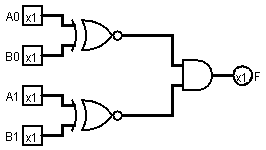
\includegraphics[width=0.3\textwidth]{5.16.png}
    \caption{5.16}
\end{figure}
}

\question{5.22}{
用与非门设计报警逻辑电路：设备中有四个传感器A、B、C、D，如果传感器A输出为\textbf{1}，同时B、C、D中至少有两个输出也为\textbf{1}，表示设备工作状态正常，否则工作异常，发出报警。
}

\solution{
$ Y = \overline{A(BC + BD + CD)} = \overline{A} + \overline{B}\,\overline{C} + \overline{B}\,\overline{D} + \overline{C}\,\overline{D} = \overline{\overline{\overline{A}} \cdot \overline{\overline{B}\,\overline{C}} \cdot \overline{\overline{B}\,\overline{D}} \cdot  \overline{\overline{C}\,\overline{D}}}$

\begin{figure}[]
    \centering
    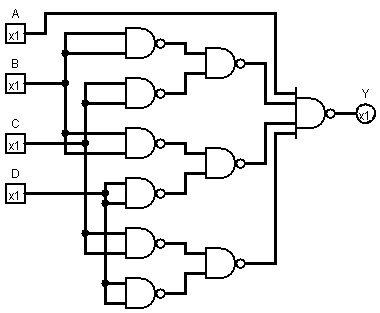
\includegraphics[width=0.3\textwidth]{5.22.png}
    \caption{5.22}
\end{figure}
}


% ============================================

\end{document}